\documentclass[a4paper,11pt]{article}
\pdfoutput=1 % if your are submitting a pdflatex (i.e. if you have
             % images in pdf, png or jpg format)

\usepackage{jheppub} % for details on the use of the package, please
                     % see the JHEP-author-manual

\usepackage[T1]{fontenc} % if needed
\usepackage{kotex}
\usepackage{hhline}

\title{\boldmath HW6 - Radio Cross Match}


%% %simple case: 2 authors, same institution
%% \author{A. Uthor}
%% \author{and A. Nother Author}
%% \affiliation{Institution,\\Address, Country}

% more complex case: 4 authors, 3 institutions, 2 footnotes
\author{김태근, 윤한결, 강호철, 송진화}

% The "\note" macro will give a warning: "Ignoring empty anchor..."
% you can safely ignore it.

\affiliation{연세대학교 천문우주학과 F조}



\begin{document} 
\maketitle
\flushbottom

\section{BPT Diagram of Non-radio-active galaxies}


\begin{figure}[h]
\centering
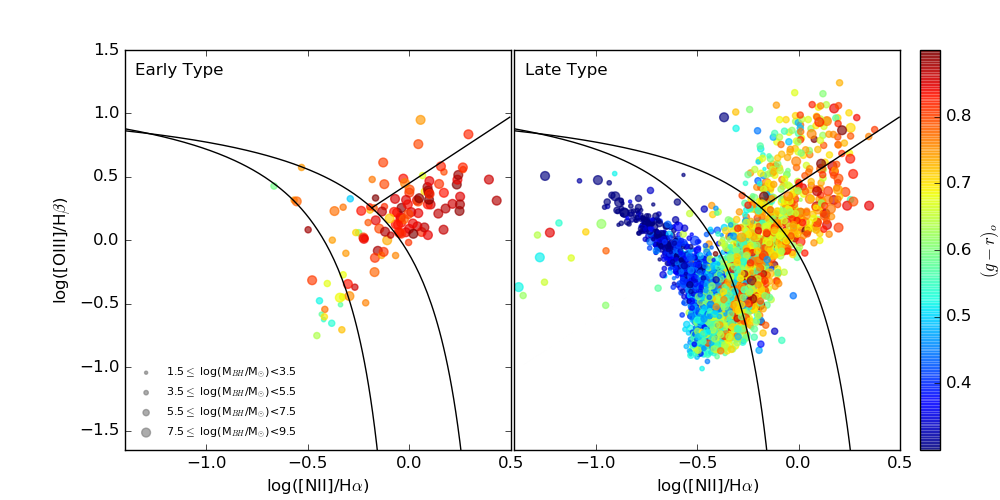
\includegraphics[height=50mm, width=100mm]{BPT.png}
\hfill
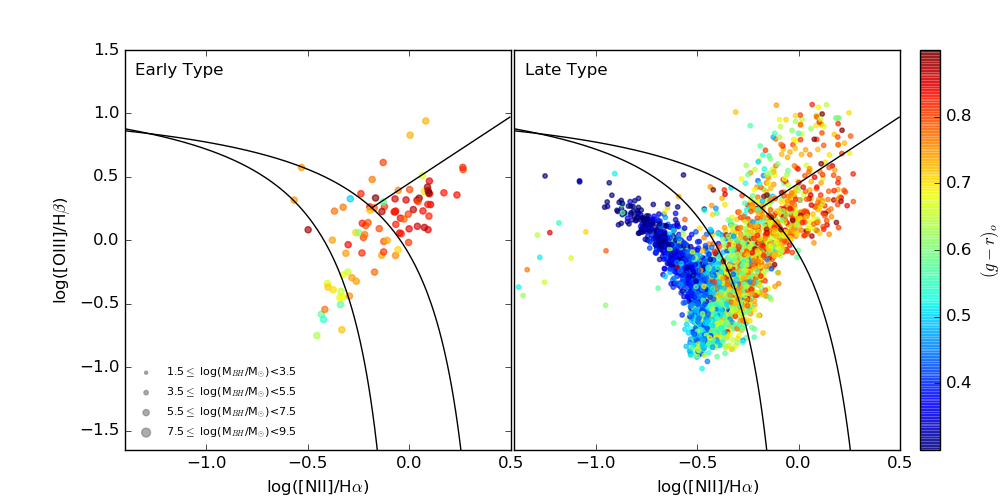
\includegraphics[height=50mm, width=100mm]{BPT_nonradio.png}
\caption{\label{fig:i} BPT Diagram of all galaxies and non-radio-active galaxies}
\end{figure}

저번 과제의 데이터 (OSSY database) 와 VLA 에서 받은 Data를 Matching시켜서 전파가 관측된 것과 아닌 것으로 나누어 BPT diagram을 그렸다. 위의 그림\ref{fig:i} 이 
저번의 BPT diagram (위쪽 그래프) 와 전파가 관측되지 않은 은하들의 BPT diagram (아래쪽 그래프)을 잘 보여주고 있다. 언뜻 보기엔 두 그래프의 양상이 상당히 흡사해보인다.
그러나 자세히보면 명백한 차이점을 볼 수 있다. 일단 전체적으로는 그래프가 왼쪽 아래로 치우쳤다. 이는 우측 위, 즉, AGN 영역이 줄어들었다는 것을 의미하는데
AGN에서는 전파가 방출되니 당연한 결과이다. 반대로 Star Forming 영역은 거의 없어지지 않고 흡사한데, 따라서 우리는 Star forming 과정은 Radio-active 하지 않다는 것을 알 수 있다.
그리고 상대적으로 점의 크기가 작아졌는데, 이는 전파를 방출하는 은하들이 대부분 Massive 한 Black hole을 가지고 있음을 의미한다. 

\section{BPT Diagram of Radio-active galaxies}

\begin{figure}[h]
\centering
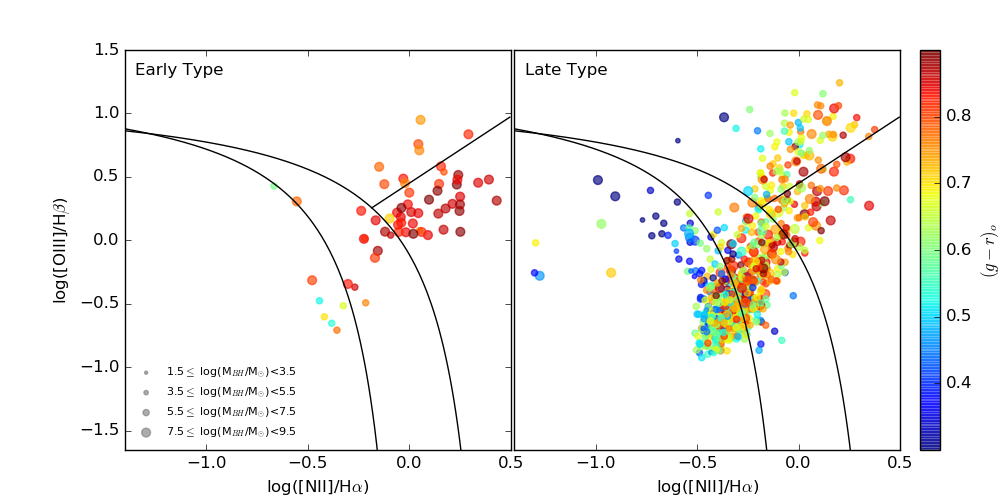
\includegraphics[height=50mm, width=100mm]{BPT_radio_Active.png}
\caption{\label{fig:ii} BPT Diagram of radio-active galaxies}
\end{figure}

우리조에서 분류한 radio-active한 Early type galaxy는 총 63개이며 그 중 Star forming region이 7개, Composite region 38, LINER가 36개, Seyfert region이 8개이다.
radio-active한 Late type galaxy는 총 730개이며 SF가 319개, Composite이 88, Seyfert가 94개, LINER가 64개이다. radio-active Early type의 특징으로 Seyfert보다 LINER가 더 많은 것을 
들 수 있는데, LINER의 스펙트럼은 starburst galaxy의 스펙트럼과 비슷한 형태인 것을 보아 이에 의한 emission line일 가능성이 있다.
하지만 starburst에 의한 line 이외의 흡수선 또한 관측되기 때문에 단지 starburst가 유일한 설명은 되지 못한다. radio-active Late type은 Late type galaxy의 특성상 가스가 많고 
star forming이 활발하기 때문에 개체수가 Early type에 비해 많고 star forming region에 분포하고 있는 은하의 수가 많다. 

\section{BPT Diagram of FR2 Galaxies}

\begin{figure}[h]
\centering
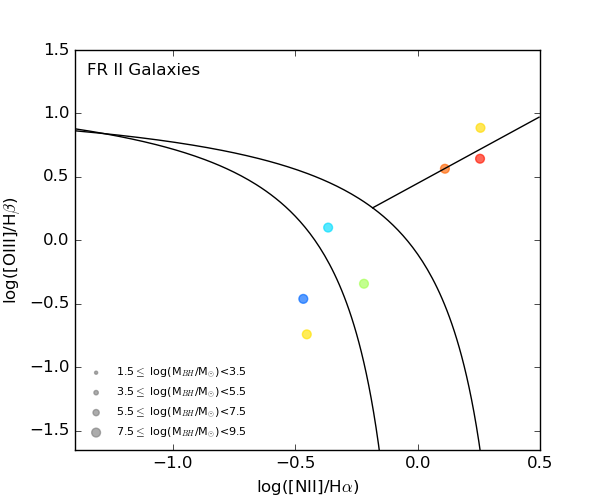
\includegraphics[height=50mm, width=60mm]{BPT_frII.png}
\caption{\label{fig:iii} BPT Diagram of FRII galaxies}
\end{figure}

Fanaroff-Riley classification에 의해 중심부 부분이 밝은 것을 FR1, 가장자리 부분이 밝은 것을 FR2로 두고 분류하였을 때 거의 대부분이 FR1으로 구분됨을 확인할 수 있었다. 
이렇게 FR2로 분류된 값들을 확인하여 보았을 때 FR2로 구분된 모든 galaxy들은 late type으로 확인되었는데, 이를 토대로 late type galaxy의 활동 정도에 대한 논의를 이끌어 낼 수 있다.
이전에 Early type과 later type의 Active Galactic Nucleus(AGN)의 차이에 대해 논의했었는데, 특히 주목해봐야 할 부분은 이번 분류를 통해 Active한 핵을 가진 거의 모든 galaxy들이 제트 방출을 관측할 수 있었다. 
즉, 제트 분출을 확인한 모든 천체들이 활동적인 핵을 확인할 수 있었다.

FR1의 경우 Early type 중 약 41\%의 galaxy가 여기에 해당하며, later type 중 16\% 정도의 galaxy가 여기에 해당한다.
그와 비고하여 재밌는 것은 위의 FR2의 경우에서 Early type과 later type의 비교에서 있다. 
위의 그래프 상에 모든 galaxy들은 late type galaxy라는 것인데 Later type의 경우 많은 양의 차가운 가스의 수축이나 압축으로 인해 생성되는 제트이며 
이 활동으로 전파가 방출되는 것으로 볼 수 있다. 

FR1의 경우에는 Early type의 경우 일반적으로 무거운 블랙홀을 포함하여 AGN을 가지게 된다는 것이며 이를 통해 전파가 방출되는 것으로 볼 수 있다.
\end{document}
